% !TEX root = ../my-thesis.tex
%
\chapter{The masses and dynamics of star clusters in the Milky Way}
\label{sec:dynamics}

\cleanchapterquote{Things are only impossible until they're not.}{Jean-Luc Picard}{(2364)}

\authorship{The results presented in this chapter will be published in Hunt and Reffert (\emph{in prep.}). All calculations, figures, and writing in this chapter were conducted by myself.}

\todo{dynamics section}

% -------------------------------------
\section{Introduction}
\label{sec:dynamics:introduction}

Five years on since the release of \gaia\ DR2 \citeme{}, the census of open clusters (OCs) has been resoundingly overhauled \citeme{tcg universe}. Thousands of new objects have been discovered, parameters have been determined to previously impossible levels of accuracy, and many OCs reported before \gaia\ have been ruled out as asterisms \citeme{multiple papers here}. However, the OC census in the age of \gaia\ remains far from perfect, and one resoundingly large issue stands out that I will attempt to address in this chapter: there is no robust observational criteria or definition for what an OC actually is.

Following up from the first major catalogue of OCs in the \gaia\ era \citeme{cantat 2018}, \citeme{cantat anders 20} conducted a search for OCs that remained undetected in \gaia\ data, and created a set of empirical observational criteria intended to split dubious objects apart from OCs. This included recommendations that a candidate OC is a clear overdensity with at least $\sim10$ member stars, a colour-magnitude diagram (CMD) that follows a clear isochrone, a median radius $r_{50}$ smaller than 15~pc and a proper motion dispersion corresponding to an upper limit no greater than 5~km\,s\textsuperscript{-1}. In their work, they used these criteria to show that a number of objects were asterisms.

However, in \citeme{paper 2} (hereafter Paper 2), in which we constructed the largest catalogue of OCs to date from a blind search using \gaia\ DR3 data \citeme{DR3}, we found that these observational criteria were too permissive, with many of the objects we detect that pass these criteria being visually much more reminiscent of moving groups (MGs). As a thought experiment, one can  This creates an awkward situation where our Paper 2 catalogue is challenging to use in many respects, with simple queries of the catalogue (particularly within a few hundred pc of the Sun where MGs are most common) returning mostly MGs. 

More accurate determination of whether or not a given object is a real bound cluster 



% PLAN
% - Masses are useful! Dynamics are useful! They're comparable to theory and represent measurements of fundamental (physical) parameters of OCs.
% - BUT: very limited measurements so far of these parameters.
% - Difficult to define OCs robustly without them (Hunt & Reffert 2023)
% - Empirical cuts on parameters insufficient to measure them.
% - MASSES: can be measured more or less two ways: counting stars or tidal parameters
% - discuss pros and cons of each way
% - DYNAMICS: some progress in studying for OCs in MW, but generally for small numbers of clusters only.
% - most clusters found to be supervirial. really?? what about as function of cluster mass, age, etc?
% - finally: masses useful for e.g. analysis of sample completeness. is a more fundamental physical parameter than the observed number of stars
% - give overview of what's in this chapter
% - emphasise that I'll be 


% -------------------------------------
\section{Mass calculations}
\label{sec:dynamics:masses}

% PLAN
% - give a quick overview of what's in this methods section


\subsection{Inference of stellar primary masses}
\label{sec:dynamics:masses:isochrones}

\begin{figure}[t]
    \centering
    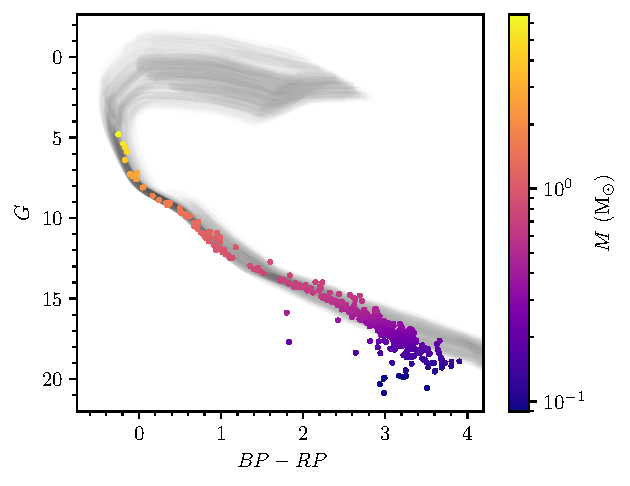
\includegraphics[width=0.8\textwidth]{fig/c4/masses_stellar.pdf}
    \caption[TODO]{TODO}
    \label{fig:dynamics:masses:stellar_masses}
 \end{figure}


\subsection{Correction for selection effects}
\label{sec:dynamics:masses:selection}

\begin{figure}[p]
    \centering
    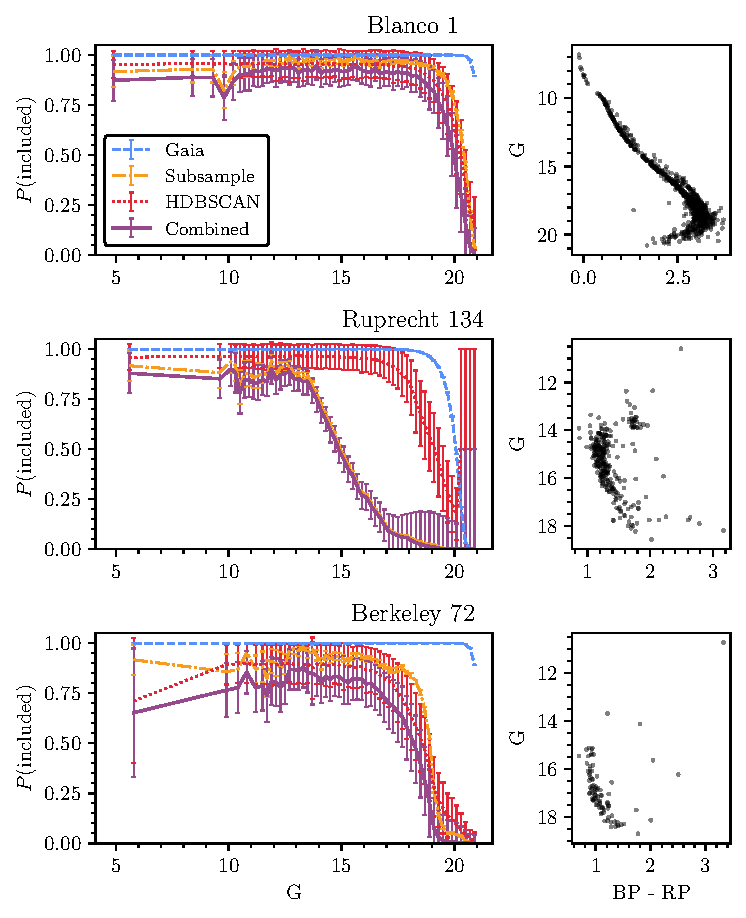
\includegraphics[width=\textwidth]{fig/c4/mass_selection_functions.pdf}
    \caption[TODO]{TODO}
    \label{fig:dynamics:masses:selection_effects}
 \end{figure}


\subsection{Correction for binaries}
\label{sec:dynamics:masses:binaries}


\subsection{Mass function fits}
\label{sec:dynamics:masses:imf_fits}

\begin{figure}[p]
    \centering
    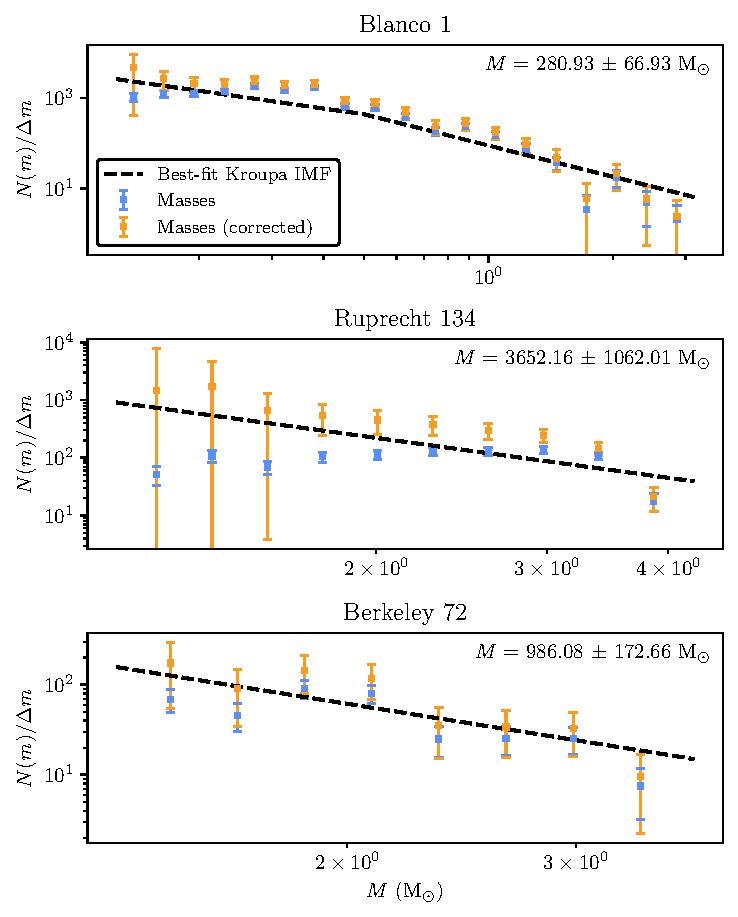
\includegraphics[width=\textwidth]{fig/c4/mass_functions.pdf}
    \caption[TODO]{TODO}
    \label{fig:dynamics:masses:mass_functions}
 \end{figure}


\subsection{Jacobi radius inference}
\label{sec:dynamics:masses:jacobi}

\begin{figure}[t]
    \centering
    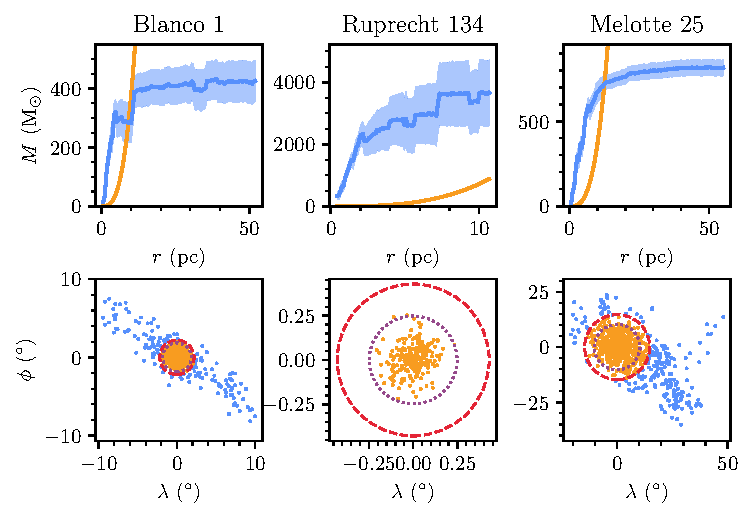
\includegraphics[width=\textwidth]{fig/c4/masses_jacobi_radii.pdf}
    \caption[TODO]{TODO}
    \label{fig:dynamics:masses:radii}
 \end{figure}



% -------------------------------------
\section{Velocity dispersion inference}
\label{sec:dynamics:velocities}


\subsection{Gaussian velocity dispersion model}
\label{sec:dynamics:velocities:model}


\subsection{Coordinate frame and radial velocity corrections}
\label{sec:dynamics:velocities:correction}


\subsection{Binary star contamination}
\label{sec:dynamics:velocities:binaries}

\begin{figure}[t]
    \centering
    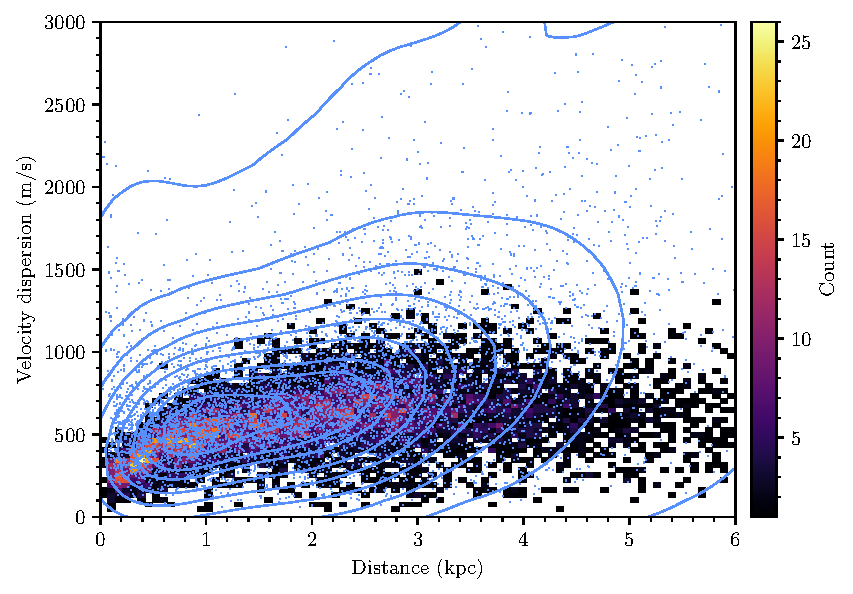
\includegraphics[width=\textwidth]{fig/c4/dispersion_binaries.pdf}
    \caption[TODO]{TODO}
    \label{fig:dynamics:velocities:binary_contamination}
 \end{figure}


% -------------------------------------
\section{Results}
\label{sec:dynamics:results}


\subsection{Masses}
\label{sec:dynamics:results:masses}

\begin{figure}[t]
    \centering
    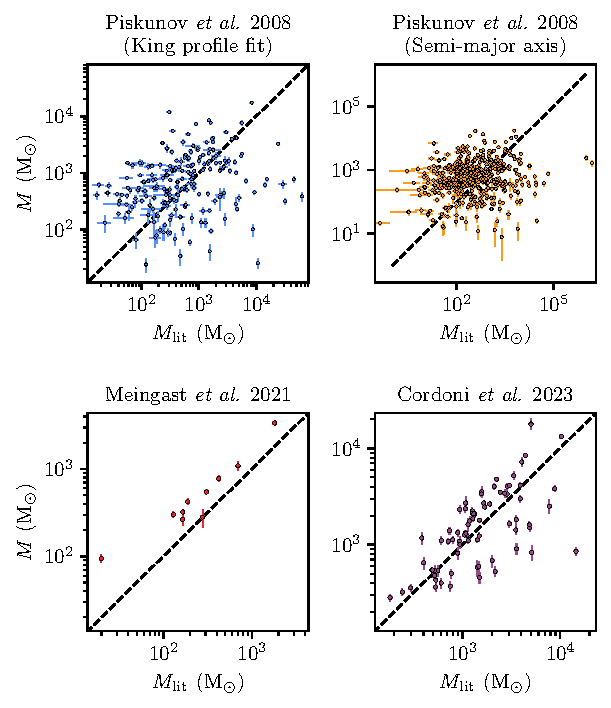
\includegraphics[width=\textwidth]{fig/c4/results_mass_comparison.pdf}
    \caption[TODO]{TODO}
    \label{fig:dynamics:results:mass_comparison}
 \end{figure}


\subsection{Jacobi radii}
\label{sec:dynamics:results:radii}

\begin{figure}[t]
    \centering
    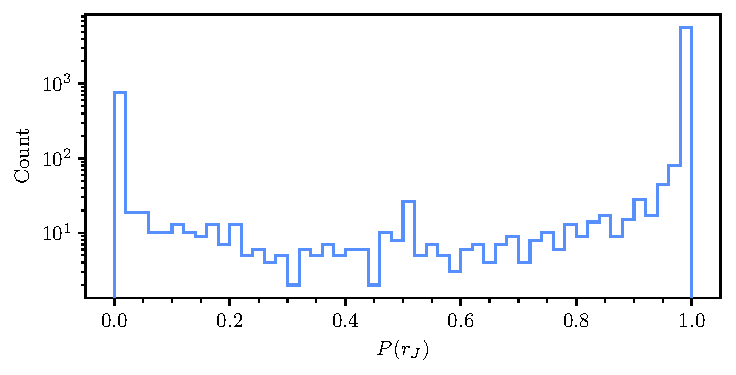
\includegraphics[width=\textwidth]{fig/c4/results_p_jac_distribution.pdf}
    \caption[TODO]{TODO}
    \label{fig:dynamics:results:jacobi_radii_distribution}
 \end{figure}


\subsection{Virial ratios}
\label{sec:dynamics:results:virial}

\begin{figure}[t]
    \centering
    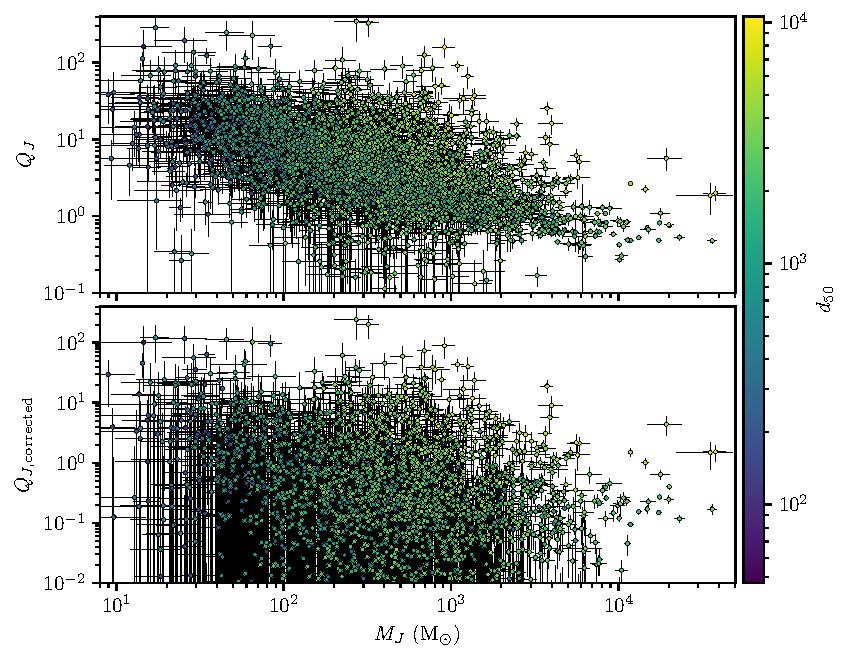
\includegraphics[width=\textwidth]{fig/c4/results_virial_vs_mass.pdf}
    \caption[TODO]{TODO}
    \label{fig:dynamics:results:virial_vs_mass}
 \end{figure}

\begin{figure}[t]
    \centering
    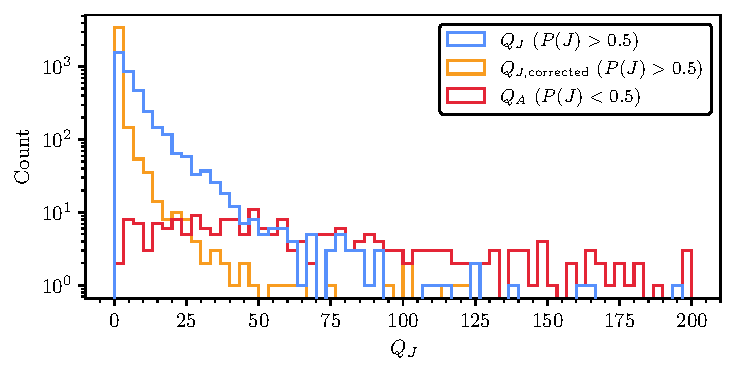
\includegraphics[width=\textwidth]{fig/c4/results_q_distribution.pdf}
    \caption[TODO]{TODO}
    \label{fig:dynamics:results:virial_ratio_distribution}
 \end{figure}


\subsection{An updated observational definition of open clusters}
\label{sec:dynamics:results:definition}

\begin{table}[t]

% Define first header
\caption{\label{tab:dynamics:catalogue_results}TODO}

\centering
\begin{tabular}{lcc}
\hline\hline
Type & Criteria & Identifier & Count \\
\hline

OC & $P(r_J) > 0.5$ and $M_J < 50$ \MSun & & TODO \\
- bound OC & $Q_{J,\text{corrected}} \leq 10$ & \texttt{o} & TODO \\
- dissolving OC & $Q_{J,\text{corrected}} \geq 10$ & \texttt{od} & TODO \\
- unbound OC? & $Q_{J,\text{corrected}} \geq 50$ & \texttt{ou} & TODO \\
\hline
MG & $P(r_J) > 0.5$ or $M_J < 50$ & & TODO \\
- without Jacobi component & $P(r_J) < 0.5$ & \texttt{m} & TODO \\
- with Jacobi component & $P(r_J) > 0.5$ & \texttt{mj} & TODO \\
\hline
GC & in \citeme{Vasiliev} & \texttt{g} & TODO \\
\hline

\end{tabular}

% \tablefoot{
% \tablefoottext{a}{}
% }

\end{table}    


% -------------------------------------
\section{Discussion}
\label{sec:dynamics:discussion}


\subsection{Completeness of the \gaia\ DR3 open cluster census}
\label{sec:dynamics:results:completeness}


% -------------------------------------
\section{Conclusions and areas for improvement before publication}
\label{sec:dynamics:conclusion}
